
\begin{figure}
	\centering
\begin{tikzpicture}[scale = 8]
\tikzstyle{VertexStyle} = []
\tikzstyle{EdgeStyle} = []
\tikzstyle{labeledStyle}=[shape = circle, minimum size = 6pt, inner sep = 1.2pt, draw]
\tikzstyle{unlabeledStyle}=[shape = circle, minimum size = 6pt, inner sep = 1.2pt, draw, fill]
\Vertex[style = labeledStyle, x = 0.650, y = 0.550, L = \small {$0$}]{v0}
\Vertex[style = labeledStyle, x = 0.850, y = 0.700, L = \small {$0$}]{v1}
\Vertex[style = labeledStyle, x = 1.050, y = 0.550, L = \small {$0$}]{v2}
\Vertex[style = labeledStyle, x = 0.850, y = 0.950, L = \small {$1$}]{v3}
\Vertex[style = labeledStyle, x = 0.750, y = 0.750, L = \small {$0$}]{v4}
\Edge[label = \tiny {}, labelstyle={auto=right, fill=none}](v1)(v0)
\Edge[label = \tiny {}, labelstyle={auto=right, fill=none}](v1)(v2)
\Edge[label = \tiny {}, labelstyle={auto=right, fill=none}](v2)(v0)
\Edge[label = \tiny {}, labelstyle={auto=right, fill=none}](v4)(v0)
\Edge[label = \tiny {}, labelstyle={auto=right, fill=none}](v4)(v3)
\Edge[label = \tiny {}, labelstyle={auto=right, fill=none}](v3)(v1)
\Edge[label = \tiny {}, labelstyle={auto=right, fill=none}](v3)(v2)
\end{tikzpicture}
\label{fig:SubdividedK4}
~~~
\begin{tikzpicture}[scale = 8]
\tikzstyle{VertexStyle} = []
\tikzstyle{EdgeStyle} = []
\tikzstyle{labeledStyle}=[shape = circle, minimum size = 6pt, inner sep = 1.2pt, draw]
\tikzstyle{unlabeledStyle}=[shape = circle, minimum size = 6pt, inner sep = 1.2pt, draw, fill]
\Vertex[style = labeledStyle, x = 0.650, y = 0.550, L = \small {$0$}]{v0}
\Vertex[style = labeledStyle, x = 0.850, y = 0.700, L = \small {$0$}]{v1}
\Vertex[style = labeledStyle, x = 1.050, y = 0.550, L = \small {$0$}]{v2}
\Vertex[style = labeledStyle, x = 0.850, y = 0.950, L = \small {$1$}]{v3}
\Vertex[style = labeledStyle, x = 0.750, y = 0.750, L = \small {$0$}]{v4}
\Vertex[style = labeledStyle, x = 0.950, y = 0.750, L = \small {$0$}]{v5}
\Edge[label = \tiny {}, labelstyle={auto=right, fill=none}](v1)(v0)
\Edge[label = \tiny {}, labelstyle={auto=right, fill=none}](v1)(v2)
\Edge[label = \tiny {}, labelstyle={auto=right, fill=none}](v2)(v0)
\Edge[label = \tiny {}, labelstyle={auto=right, fill=none}](v4)(v0)
\Edge[label = \tiny {}, labelstyle={auto=right, fill=none}](v4)(v3)
\Edge[label = \tiny {}, labelstyle={auto=right, fill=none}](v5)(v2)
\Edge[label = \tiny {}, labelstyle={auto=right, fill=none}](v5)(v3)
\Edge[label = \tiny {}, labelstyle={auto=right, fill=none}](v3)(v1)
\end{tikzpicture}
	\caption{The pair $(G,h_x)$ is AT, when $G$ is formed from $K_4$ by subdividing
one or two edges incident to $x$.}
	\label{fig:TriangleRuinsPath}
\end{figure}

\begin{figure}
	\centering
%
\begin{tikzpicture}[scale = 8]
\tikzstyle{VertexStyle} = []
\tikzstyle{EdgeStyle} = []
\tikzstyle{labeledStyle}=[shape = circle, minimum size = 6pt, inner sep = 1.2pt, draw]
\tikzstyle{unlabeledStyle}=[shape = circle, minimum size = 6pt, inner sep = 1.2pt, draw, fill]
\Vertex[style = labeledStyle, x = 0.650, y = 0.550, L = \small {$0$}]{v0}
\Vertex[style = labeledStyle, x = 0.850, y = 0.700, L = \small {$0$}]{v1}
\Vertex[style = labeledStyle, x = 1.050, y = 0.550, L = \small {$0$}]{v2}
\Vertex[style = labeledStyle, x = 0.850, y = 0.950, L = \small {$1$}]{v3}
\Vertex[style = labeledStyle, x = 0.850, y = 0.600, L = \small {$0$}]{v4}
\Edge[label = \tiny {}, labelstyle={auto=right, fill=none}](v1)(v0)
\Edge[label = \tiny {}, labelstyle={auto=right, fill=none}](v1)(v2)
\Edge[label = \tiny {}, labelstyle={auto=right, fill=none}](v1)(v3)
\Edge[label = \tiny {}, labelstyle={auto=right, fill=none}](v2)(v0)
\Edge[label = \tiny {}, labelstyle={auto=right, fill=none}](v3)(v0)
\Edge[label = \tiny {}, labelstyle={auto=right, fill=none}](v3)(v2)
\Edge[label = \tiny {}, labelstyle={auto=right, fill=none}](v4)(v1)
\Edge[label = \tiny {}, labelstyle={auto=right, fill=none}](v4)(v0)
\Edge[label = \tiny {}, labelstyle={auto=right, fill=none}](v4)(v2)
\end{tikzpicture}
~~~
\begin{tikzpicture}[scale = 8]
\tikzstyle{VertexStyle} = []
\tikzstyle{EdgeStyle} = []
\tikzstyle{labeledStyle}=[shape = circle, minimum size = 6pt, inner sep = 1.2pt, draw]
\tikzstyle{unlabeledStyle}=[shape = circle, minimum size = 6pt, inner sep = 1.2pt, draw, fill]
\Vertex[style = labeledStyle, x = 0.650, y = 0.550, L = \small {$0$}]{v0}
\Vertex[style = labeledStyle, x = 0.850, y = 0.700, L = \small {$0$}]{v1}
\Vertex[style = labeledStyle, x = 1.050, y = 0.550, L = \small {$0$}]{v2}
\Vertex[style = labeledStyle, x = 0.850, y = 0.950, L = \small {$1$}]{v3}
\Vertex[style = labeledStyle, x = 0.750, y = 0.750, L = \small {$0$}]{v4}
\Vertex[style = labeledStyle, x = 0.850, y = 0.800, L = \small {$0$}]{v5}
\Vertex[style = labeledStyle, x = 0.950, y = 0.750, L = \small {$0$}]{v6}
\Vertex[style = labeledStyle, x = 0.850, y = 0.600, L = \small {$0$}]{v7}
\Edge[label = \tiny {}, labelstyle={auto=right, fill=none}](v1)(v0)
\Edge[label = \tiny {}, labelstyle={auto=right, fill=none}](v1)(v2)
\Edge[label = \tiny {}, labelstyle={auto=right, fill=none}](v2)(v0)
\Edge[label = \tiny {}, labelstyle={auto=right, fill=none}](v4)(v0)
\Edge[label = \tiny {}, labelstyle={auto=right, fill=none}](v4)(v3)
\Edge[label = \tiny {}, labelstyle={auto=right, fill=none}](v5)(v1)
\Edge[label = \tiny {}, labelstyle={auto=right, fill=none}](v5)(v3)
\Edge[label = \tiny {}, labelstyle={auto=right, fill=none}](v6)(v2)
\Edge[label = \tiny {}, labelstyle={auto=right, fill=none}](v6)(v3)
\Edge[label = \tiny {}, labelstyle={auto=right, fill=none}](v7)(v1)
\Edge[label = \tiny {}, labelstyle={auto=right, fill=none}](v7)(v0)
\Edge[label = \tiny {}, labelstyle={auto=right, fill=none}](v7)(v2)
\end{tikzpicture}
%		\caption{This is AT.}
		\label{fig:thebigone}
	\caption{(a) The pair $(G,h_x)$ is AT, where $G=K_5-xy$. 
%and $x$ is an endpoint of the missing edge. 
(b) The pair $(G,h_x)$ is AT, where $G$ is formed from $K_5-e$ by
subdividing each edge incident to $x$.}
	\label{fig:K5minus}
\end{figure}
